\subsection{Restriction and Prolongation operations}

Until this moment we have not talked about the grid size $N_x$ and $N_y$.  We only allow the grid size to be a power of two to make things as simply as possible.

\begin{equation}
2^M = max(N_x, N_y)
\end{equation}
\noindent
Before we break down the multigrid algorithm itself, we need a method to go from a matrix $Q^M$ with resolution $N_x,N_y$ to a lower resolution matrix $Q^{M-1}$ with dimensions half the size, i.e. $N_x/2,N_y/2$. In general, we need an operation that uses a matrix $Q^{M-m}$ with dimensions $\frac{N_x}{2^m}$ as an input and produces a down-scaled matrix $Q^{M-m-1}$. We call this operation restriction. We will use bilinear interpolation for downscaling a matrix.

\begin{equation}
Q^{M-n-1}_{i,j} = \frac{1}{4} ( Q^{M-n}_{2i,2j} + Q^{M-n}_{2i + 1,2j} + Q^{M-n}_{2i + 1,2j +1 }  + Q^{M-n}_{2i,2j + 1} )
\label{restricteq}
\end{equation}
\noindent
Figure \ref {restrict} gives a numerical example of the restriction operation seen in Equation \ref{restricteq}
\begin{figure}[ht!]
\centering
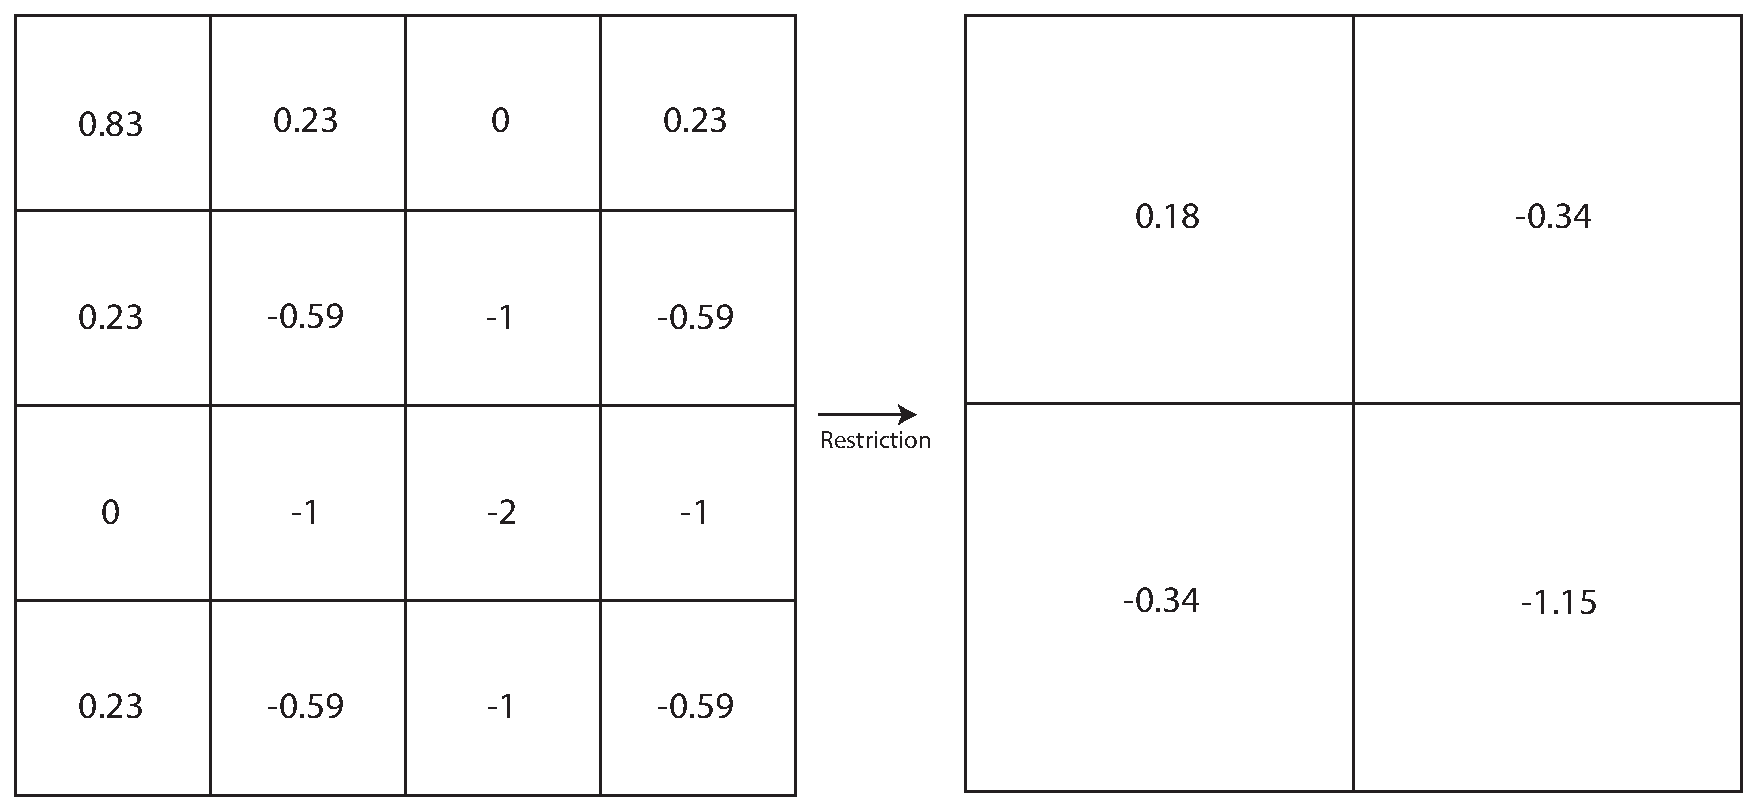
\includegraphics[width=120mm]{img/restrict.pdf}
\caption{A numerical example of the restriction operation.}
\label{restrict}
\end{figure}
\newline
\noindent
To keep things simple, we also use bilinear interpolation in the prolongation operator where we do the opposite from restriction, i.e. go from matrix $Q^{M-m}$ to matrix $Q^{M-m+1}$. Although using the same interpolation scheme, prolongation is a bit trickier to get right since the indices are not aligned up as perfect as in the restriction operator. Figure \ref {prolong} demonstrates why the indices are aligned slightly awkward.

\begin{figure}[ht!]
\centering
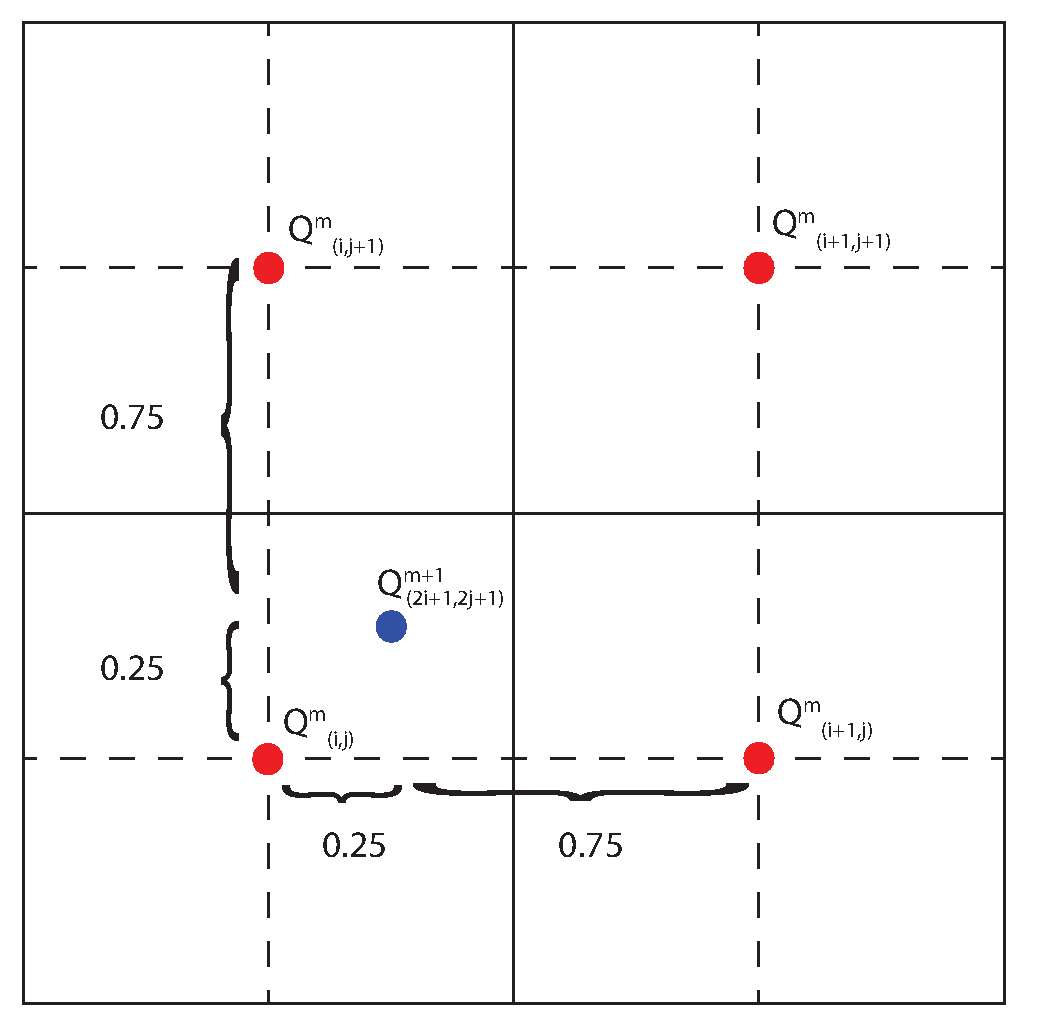
\includegraphics[width=80mm]{img/prolong.pdf}
\caption{Barycentric coordinates are used to determine bilinear interpolation in the prolongation operator.}
\label{prolong}
\end{figure}
\noindent
The center of a cell in grid $Q^{M-n}$ gives us the barycentric coordinates between nearby values in $Q^{M-n-1}$ as can be seen in Figure \ref{prolong}. This gives us the following scheme for the prolongation operator:

\begin{equation}
\begin{split}
Q^{M-n}_{2i,2j} &= \frac{1}{16} Q^{M-n-1}_{i-1,j-1} +  \frac{3}{16} Q^{M-n-1}_{i-1,j} +  \frac{3}{16} Q^{M-n-1}_{i,j-1}+  \frac{9}{16} Q^{M-n-1}_{i,j} \\ 
Q^{M-n}_{2i + 1,2j} &= \frac{1}{16} Q^{M-n-1}_{i+1,j-1} +  \frac{3}{16} Q^{M-n-1}_{i,j-1} +  \frac{3}{16} Q^{M-n-1}_{i+1,j}+  \frac{9}{16} Q^{M-n-1}_{i,j} \\ 
Q^{M-n}_{2i,2j+1} &= \frac{1}{16} Q^{M-n-1}_{i-1,j+1} +  \frac{3}{16} Q^{M-n-1}_{i-1,j} +  \frac{3}{16} Q^{M-n-1}_{i,j+1}+  \frac{9}{16} Q^{M-n-1}_{i,j} \\ 
Q^{M-n}_{2i+1,2j+1} &= \frac{1}{16} Q^{M-n-1}_{i+1,j+1} +  \frac{3}{16} Q^{M-n-1}_{i+1,j} +  \frac{3}{16} Q^{M-n-1}_{i,j+1}+  \frac{9}{16} Q^{M-n-1}_{i,j} \\ 
\end{split}
\label{prolongeq}
\end{equation}
\noindent
Equation \ref{prolongeq} only works if the updated cells are not on the boundary and has four neighboring cells in the lower dimension grid. If the cell is on the boundary, we use simple linear interpolation between the two cells in $Q^{M-n-1}$ with weights $0.75$ and $0.25$. There is one last special case. At the four corners, we use the same value as the corners of the lower dimension grid since there is nothing nearby to interpolate from.
